\chapter{Optimal scenario tree selection}
\label{chapter4}
In this chapter we propose an experiment to find the optimal scenario tree structure.
\section{Methods}
The whole implementation was programmed in Python \cite[Version 3.11]{python}, mathematical optimization problems were implemented in GAMS \cite[version]{GAMS} \todo{add version of gams} using the Python API. Data were sourced from \cite{yahoo} using the \cite[version 0.1.74]{yfinance} package. The reinforcement learning agent was implemented using the \textit{Stable~baselines~3} package \cite[version 1.6.2]{stable_baselines3} and the environment was implemented using the \textit{gym} package \cite[version 0.21.0]{openai_gym}.

\section{Data}
For our experiments, we used data obtained from \cite{yahoo} using the \cite[version 0.1.74]{yfinance} package. We downloaded historical asset price data from 1.1.2000 to 31.12.2019 for 49 financial stocks given in Table \ref{table:stock_tickers_used}. We split this data into four sets by splitting the data into two sets by time, set \textit{train} (from 1.1.2000 to 31.12.2009) and set \textit{test} (from 1.1.2009 to 31.12.2009) and splitting the stock tickers into set $A$, see Table \ref{table:stock_tickers_in_set_A} and set $B$, see Table \ref{table:stock_tickers_in_set_B}. This yielded us four distinct sets:
\begin{itemize}
\item (\textit{train}, $A$),
\item (\textit{test}, $A$),
\item (\textit{train}, $B$),
\item (\textit{test}, $B$).
\end{itemize}
We trained the agent on the set (\textit{time train}, $A$) and evaluate its performance on the other three sets, to evaluate whether the agent is able to:
\begin{enumerate}
\item generalise to unseen stocks in the same period,
\item generalise to the same stocks in the future,
\item generelise to unseen stocks in the future.
\end{enumerate}

For the problem to make sense, we needed to obtain data for the moment matching method in such a way that the scenario trees were constructed in such a way that the investment horizon was the same independent of the depth. This was achieved by splitting the investment period into equisized parts based on the number of stages of the tree.
The moment matching method uses estimated moments from the dataset. For a scenario tree with 3 stages, the approach outlined above would split the investment period into just 3 periods and we would thus obtain only 3 realisations of simple returns, which means that the sample moments would not be very precise. To counteract this effect, we chose to split the investment period into $4*number\_stages$ periods, calculate the simple returns and estimate the sample moments and correlations from this larger sample. Practically, this means that we have shortened the investment horizon from 10 years to 2.5 years. 

\section{Environment}
For the purposes of training the reinforcement agent to choose the best scenario tree structure, we adapted the well known GridWorld environment to represent iterative stage by stage building of the scenario tree.
\begin{rem}
The GridWorld environemnt is a well known introductory environment for training reinforcement learning agents. It consists of a $n$ by $n$ grid, where the agent starts on a given tile (a position on the grid, i.e. for example the bottom left corner) and must reach a target tile and upon reaching the tile, it receives a reward. The agent can perform 4 actions -- move up, move down, move left and move right. None of the tiles apart from the target tile return rewards. Optionally, if we want the agent to reach the target in the least moves possible, a small constant negative reward can be assigned to each step the agent takes.
\end{rem}
We designed and implemented a custom GridWorld environment, which we call TreeBuildingEnv.

\subsection{TreeBuildingEnv}
TreeBuildingEnv is an adaptation of the GridWorld environment to allow the agent to build scenario trees based on given predictors. 
The state is given as a 8 by 8 tree building grid (which starts filled with zeros only in the initial state) and the set of 9 predictors. The set of predictors is obtained at the beginning of each episode and is constant throughout the episode. Each row in the tree building grid represents part of the tree building process. The first row corresponds to the chosen depth of the tree. The following rows each represent the chosen branching (number of children) in each stage, from the first to last.

 In each state, the agent can take any action in the set $\{3,4,5,6,7\}$, which we from now on refer to as \textit{action set}. In the initial state, we allow the agent to perform only actions $\{3,4,5\}$ from the action set to choose the depth of tree and upon performing any of these actions, 1 is placed at the corresponding position in the first row. If the agent chooses action 6 or 7, it is forced to perform action 5. \todo{add footnote that links to computational difficulties, why are we forcing the action?}


\begin{figure}[H]
  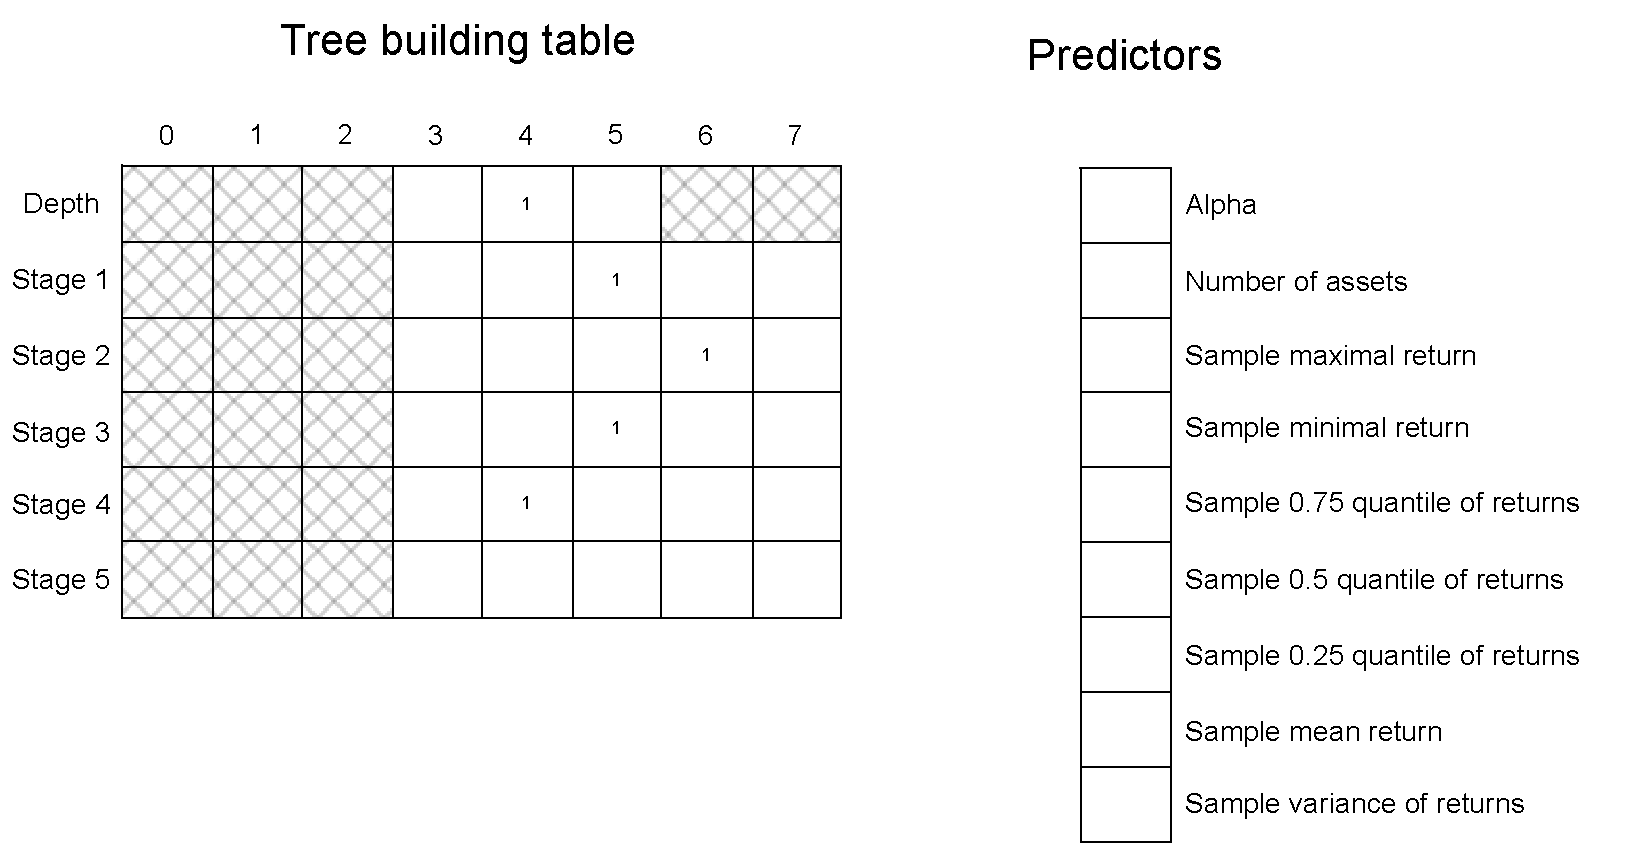
\includegraphics[width=\linewidth]{../img/Treebuildingenv_graph.pdf}
  \caption{TreeBuildingEnv. State illustration when a 4 stage tree is generated with successive branching [5,6,5,4]. Crosshatching represents invalid actions. Predictors are represented as an empty array, in reality they are populated with numerical data on the whole period returns, see Section \ref{subsection:predictors}.}
  \label{fig:treebuildingenv}
\end{figure}


In the following states, where the agent chooses the branching in each stage, the agent can perform any action in the action set and again upon performing each action, 1 is placed at position action in the next row (if the action is valid). To obtain reasonable trees, we had to constrain the size of the tree the agent can take (the maximum number of scenarios). We always require that the tree must have atleast 100 scenarios and at most 700. In each model building stage, we check if it is possible to perform the chosen action such that a final tree that remains within these limits is possible. If it is not possible, the action is considered invalid and the agent is forced to take the maximum valid action (where valid action refers to any action for which building a tree that stays in the given limits is possible). In case the chosen action was invalid, 1 is placed at the position of the forced maximum valid action.

When the agent has taken as many actions as the chosen depth of tree, the episode ends, the mean CVaR problem is solved using the given scenario tree structure and the obtained reward is returned. An illustration of the environment can be found in Figure \ref{fig:treebuildingenv}.

\subsection{Predictors}
\label{subsection:predictors}
At the beginning of each episode, between 7 and 10 assets are randomly chosen (with uniform probabilities for the number of assets) from the training data and simple returns are calculated for the whole time range. $\alpha$ is randomly chosen uniformly from the set $\{0.8, 0.85, 0.9, 0.95\}$ and the following predictors are provided to the agent:
\begin{enumerate}
\item $\alpha$
\item number of sampled assets
\item maximum return
\item minimum return
\item 0.75 quantile of returns
\item 0.5 quantile of returns
\item 0.25 quantile of returns
\item mean of returns
\item variance of returns
\end{enumerate}
The predictors are then constant throught the entire episode.

\section{Implementation}
\subsection{Moment matching}
%Gülpinar N, Rustem G, Settergren R, Simulation and Optimization Ap-
%%proaches to Scenario Generatin, Journal of Economic Dynamics & Control,
%vol. 28, Elsevier Science, 2004 - Moment matching - sequential vs whole tree
We used the moment matching method in the form given in Definition \ref{defn:moment_matching_method} with one small adjustment. 

When looking at the generated scenarios, we noticed that usually, only 3 scenarios with positive probabilities were generated and the rest had almost zero probability. This would fundamentally change the properties of scenario trees that we want to explore (dependence of objective function on tree size), since then we might think we are using a large tree, which in reality is much smaller due to the scenarios with zero probability. 

To counteract this effect, we added the constraint $p_j \geq 0.1$ to the implementation of Definition \ref{defn:moment_matching_method}, which solved the problem. With the notation developed in Definition \ref{defn:moment_matching_method}, the model now reads
\begin{alignat}{10}
& && && \underset{\substack{p_j, x_{i,j}, \\ j \in \{1,...,N\}, i \in I}}{\min} \sum_{i\in I} \sum_{k\in \mathcal{M}} \left(m_{i,k} - M_{i,k}\right)^2 + \sum_{(i, i') \in I, i < i'}(c_{i,i'}-C_{i,i'})^2 \nonumber \\
& s.t. && \sum_{j=1}^N p_j&&=1 \nonumber \\
& && m_{i,1}&&=\sum_{j=1}^N p_jx_{i,j}, i \in I \nonumber \\
& && m_{i,k}&&=\sum_{j=1}^N p_j(x_{i,j}-m_{i,1})^k, i \in I, k>1 \nonumber \\
& && c_{i,i'}&&=\sum_{j=1}^N(x_{i,j}-m_{i,1})(x_{i',j}-m_{i',1})p_j, i,i' \in I, i<i' \nonumber
\end{alignat}
\vspace{-0.5cm}
\begin{alignat}{10}
& x_{i,j}^L<=x_{i,j}<=x_{i,j}^U, i \in I, j=1,\dots,N, \nonumber \\
& \frac{1}{10} <= p_j <= 1, j=1,\dots,N. \nonumber
\end{alignat}

This means that we are generating stagewise independent balanced scenario trees, where the probabilities of each child node may vary, but are at least 0.1. This may lead to the fact that we are not able to account for scenarios with very small probability, which is a limitation, as financial data distributions are generally heavy tailed.


\subsection{Mean CVaR model}
The mean CVaR model was implemented exactly as given in Equation \ref{eq:cvar_multistage_risk_aversion} using the scenario tree generated from the moment matching method.

\subsection{Reinforcement agent}
We chose to use a tried and tested implementation of state of the art algorithms in the \textit{Stable Baselines 3} \cite{stable_baselines3} library. We experimented with multiple architectures and algorithms implemented therein, particularly A2C and PPO, while eventually settling on using PPO in the results given in Section \ref{section:experimental_results}. Here we share our experience with training the reinforcement agent.

We first experimented with the algorithms using a toy environment (TreeBuildingEnv with synthetic predictors and rewards) to obtain some semblance of how long it takes to obtain a reward better than the random agent. We experimented with several neural net architectures and found out that PPO usually outperformed A2C (converged much faster) with the same neural net architecture. 

We also experimented with neural net architectures and found that even for very simple tasks (such as learning a different action based on the value of $\alpha$), a very nontrivial number of neurons in the hidden layers is required for the model to be able to solve the environment. Particularly, for a deterministic toy example where $\alpha$ was randomly sampled from the set $\{0.9, 0.95\}$ and based on the given $\alpha$ the best depth of tree to take was $3$ if $\alpha=0.9$ and $5$ if $\alpha=0.95$, the reinforcement agent didn't learn anything within hudreds of thousands of timesteps, unless we used an architecture with two hidden layers of 128 and 64 neurons respectively, where the second layer is separate for the actor and the critic heads (which estimate the policy and the action value). Furthermore, we used ReLu activations between each layer. 

Due to the results obtained from the synthetic toy environment, we decided to use a very similar architecture as given above, where the only change is that we use 256 and 128 neurons in the hidden layers instead of 128 and 64, as the task we are trying to solve is much more difficult and stochastic.

\section{Experimental results}
\label{section:experimental_results}

\section{Computational difficulties}
\label{section:computational_difficulties}
The writing of this thesis has been plagued by computational difficulties from the start and we wish to share our experience with implementing all parts of this thesis here. 

First of all, the moment matching method, which seems quite easy to implement, required a significant amount of iterations and trying different optimization frameworks and solvers to actually obtain a working implementation. We have tried several python packages with open source solvers (most notably scipy, mystic and gekko \todo{add reference} and the IPOPT solver) and none of them produced a suitable result despite correct implementation due to low strenght of the open source solvers. We finally settled on using GAMS with the CONOPT solver \todo{add reference} which worked out quite nicely. This however required us to connect our Python code to GAMS using the GAMS Python API, which meant that we could not use a compute cluster due to licensing limitations. 

Since we already had the dependence on GAMS, we also implemented the mean CVaR model in GAMS using the CPLEX solver. While the implementation itself in GAMS was not terribly difficult, bending all data in the correct way and formulating the nonanticipativity constraints correctly took significant effort.

Lastly, the reinforcement learning part. This part was plagued by slow training and therefore a significant amount of time was spent on training the models, since the dependence on GAMS didn't allow training the reinforcement agent on a compute cluster with hundreds of cores, but we were rather constrained to a personal computer with 6 cores. This was a significant limitation, since training reinforcement agents is usually very computationally intensive (e.g. the state of the art models mentioned in the beginning of Chapter \ref{chapter3} were usually trained for months on hundreds of machines).